\chapter{Shape Manipulation of Bevel-tip Needles} \label{chap:chap-4}
% \begin{itemize}
% \item Model: ICRA 2024
% \item Control: EMBC 2024
% \item Feedback: (simulated) EMBC 2024
% \end{itemize}

\section{Chapter Overview}
\label{sec:chap-4-overview}

The current chapter is based on

\parencite{wangBevelTipNeedleDeflection2024}: 

- Wang, Y., Al-Zogbi, Lidia, Liu, G., Liu, J., Tokuda, J., Krieger, A., \& Iordachita, I. (2024). Bevel-Tip Needle Deflection Modeling, Simulation, and Validation in Multi-Layer Tissues. IEEE International Conference on Robotics and Automation, IEEE International Conference on Robotics and Automation, 2024.

\parencite{wangShapeManipulationBevelTip2024}: Wang, Y., Al-Zogbi, Lidia, Liu, J., Shepard, L., Ghazi, A., Tokuda, J., Leonard, S., … (2024). Shape Manipulation of Bevel-Tip Needles for Prostate Biopsy Procedures: A Comparison of Two Resolved-Rate Controllers. In , 2024 46th Annual International Conference of the IEEE Engineering in Medicine and Biology Society (EMBC) (pp. 1–7).

\section{Modeling of Needle Shape Manipulation}
\label{sec:chap-4-model}

Bevel-tip needle insertions are often modeled using kinematic descriptions originating from the field of vehicle dynamics, where needle motions are formulated from a series of nonholonomic constraints~\parencite{parkDiffusionBasedMotionPlanning2005,websterNonholonomicModelingNeedle2006, ,alterovitzMotionPlanningUncertainty2008}. Although kinematic models can simplify needle path planning and shape prediction, their application is limited to cases where the needle is highly flexible relative to the surrounding soft tissues, and the interaction between needle shaft and soft tissues is negligible. Additionally, needle steering is typically restricted to insertion and axial rotation, while avoiding any lateral needle motion that can cause the flexible needle to bend due to soft tissue interactions, further limiting the overall generalizability of such approach.

One way to account for the interaction between the needle's shaft and soft tissue is through force modeling~\parencite{dimaioNeedleSteeringMotion2005,dimaioInteractiveSimulationNeedle2005, ,abolhassaniNeedleInsertionSoft2007,glozmanImageGuidedRoboticFlexible2007,abayazidIntegratingDeflectionModels2013, ,roesthuisMechanicsNeedleTissueInteraction,adagolodjoRoboticInsertionFlexible2019}. In planar cases, the lateral interaction between a flexible needle and soft tissue is typically represented by a linear elastic beam for the needle shaft, and distributed linear springs along the needle shaft for the tissue~\parencite{dimaioNeedleSteeringMotion2005,dimaioInteractiveSimulationNeedle2005,abolhassaniNeedleInsertionSoft2007,glozmanImageGuidedRoboticFlexible2007,abayazidIntegratingDeflectionModels2013}. For example, DiMaio and Salcudean~\parencite{dimaioNeedleSteeringMotion2005,dimaioInteractiveSimulationNeedle2005} present a mechanics-based model based on linear needle bending model coupled with a linear tissue material, and they use needle base control to guide a symmetric-tip needle to a desired location. Glozman and Shoham~\parencite{glozmanImageGuidedRoboticFlexible2007} use a distributed linear spring model to represent tissue reaction force, and their method relies on X-ray feedback to close the control loop. Roesthuis~\textit{et al.} extend the formulation to bevel tip needles by considering a transverse tip force generated by soft tissues during needle insertion~\cite{roesthuisMechanicsNeedleTissueInteraction}, and Abayazid~\textit{et al.} further enrich the formulation by considering the double-bend shape of a bevel-tip needle~\parencite{abayazidIntegratingDeflectionModels2013}. 

Notably, work done on symmetric-tip needles is primarily focused on lateral base motion to achieve needle steering; on the other hand, bevel-tip needle steering is typically achieved only by changing the bevel orientation via axial rotation, while largely ignoring lateral motion of the needle. However, in reality, both lateral base motion and needle tip bevel can be used for steering, albeit with different working principles. Furthermore, a common feature of previous works is the use of largely simplified linear tissue behavior model. Biological soft tissues exhibit highly nonlinear stress-stretch behavior, which cannot be captured by such models~\parencite{humphreyIntroductionBiomechanicsSolids2025,singhMechanicalPropertiesWholebody2021}. The lack of a realistic tissue model also makes the choice of tissue linearity measure rather arbitrary. Adagolodjo~\textit{et al.} address tissue nonlinearity in symmetric needle insertions using the SOFA framework~\parencite{adagolodjoRoboticInsertionFlexible2019}, an open-source interactive finite element physics simulator designed to provide real-time computational capabilities~\cite{SOFA_2012, SOFA_2017}. However, no model validation is provided in~\parencite{adagolodjoRoboticInsertionFlexible2019}; instead, the overall control system is evaluated, with model errors compensated for using high-frequency non-rigid tissue registration enabled by six Flex13 cameras, which is an unrealistic requirement in clinical settings.

We present 1) a mechanics-based needle-tissue interaction model for bevel-tip needle insertion that accounts for nonlinear soft tissue behaviors and multi-layer scenarios, and 2) an interactive finite element simulation that allows full three-DOF planar control inputs to be placed anywhere along the needle, enabling the simulation of various clinical scenarios. We showcase the versatility of the model and simulation with soft tissue phantoms consisting of up to four different layers, as well as non-homogeneous chicken breast tissues.

\subsection{Modeling and Simulation}
\label{sec:chap-4-modeling-and-simulation}

Our goal is to create a prototypical mechanics-based bevel tip needle insertion simulation that accounts for 1) nonlinear strain-dependent behavior of biological soft tissues under compression, 2) needle interaction with multiple soft tissue layers of varied mechanical properties, 3) multiple control inputs along the length of the needle, and 4) full three-degree-of-freedom planar needle motions such as insertion, retraction, as well as bending and in-plane rotation.

The current simulation extends previous theoretical foundation~\parencite{wangFlexibleNeedleBending2023} with the introduction of bevel effect during needle insertion as well as incorporation of multiple control inputs along the length of the needle.

\begin{figure}[ht]
  \centering
  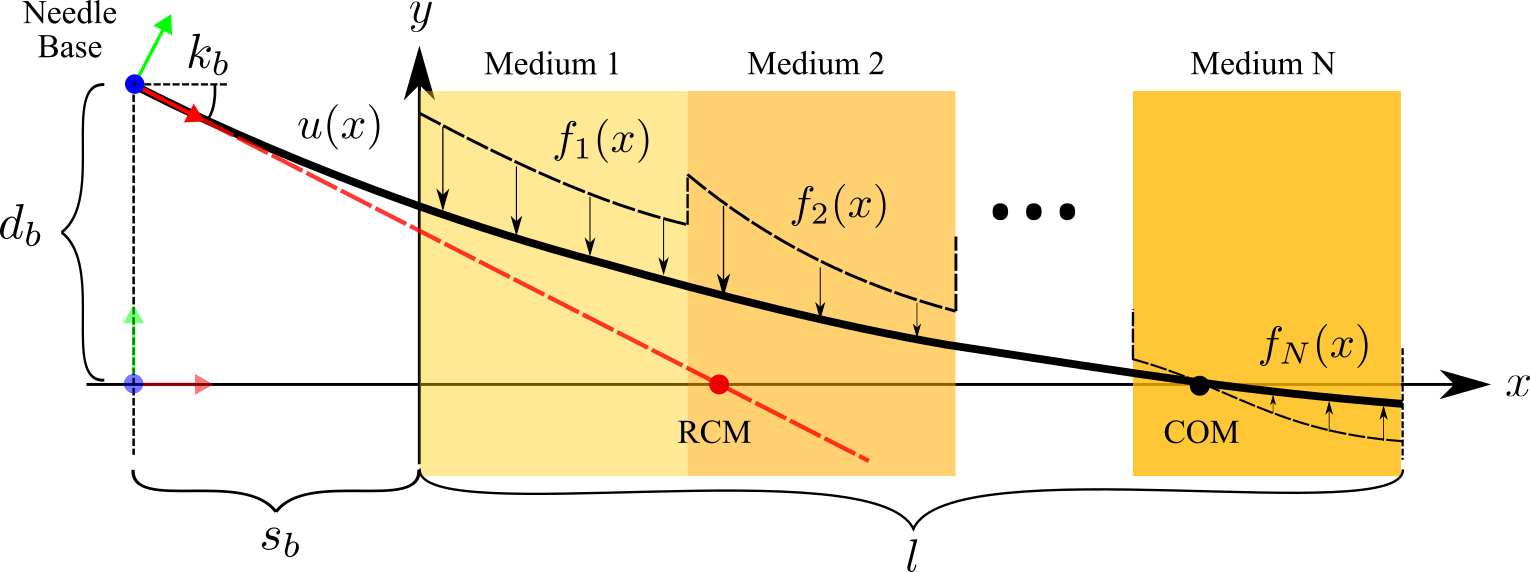
\includegraphics[width=\textwidth]{manuscripts/ICRA_2024/figures/model_schematic.png}
  \caption{Bevel tip needle insertion simulation with four layers of Ogden-type soft medium. Needle base controls horizontal ($H_1^m$) and vertical displacements and slope ($V_1^m$). A horizontally-fixed needle template (green circle) controls vertical displacement and prescribes zero slope ($V_2^m$). Contact points (blue cross) are placed dynamically, and simulate a bevel effect at the needle tip. Input steps $m\in \left\{ 1, 2, 3 \right\}$.}
  \label{fig:chap-4-model-schematic}
\end{figure}

To simulate the needle's bevel effect during insertion, an offset $b$ is applied to new contact points created at the needle tip (see~\cref{fig:chap-4-model-schematic}). This offset can correlate to the tip bevel geometry, and effectively creates a ``pre-stretched spring'' whose reaction force is tissue-dependent. By resolving the needle bending formulation in the next simulation step, the resultant tip force generated by the offset is computationally incorporated into the model, allowing the needle tip to bend in the corresponding direction. By controlling the sign and magnitude of this offset, different bevel effects can be simulated, as shown in~\cref{fig:chap-3-model-schematic}. Active needles whose tip orientation is adjustable can also be simulated by changing the offset parameter online, although such use cases are not considered in the current study~\parencite{ryuFeasibilityStudyOptically2011,karimi3DSteerableActive2019, ,padasdaoShapeMemoryAlloy2020}.

Known coordinates of the needle points can be used as control points along the needle, and are treated as essential boundary conditions for their corresponding node. For example, the needle base can have a known configuration that is robotically controlled, and the needle shaft can be constrained to move through a template.

To create an interactive simulation, we distinguish two types of user inputs: ``vertical'' $V$-input and ``horizontal'' $H$-input. $V$-input is a condition that directly affects the needle's shape, such as nodal lateral displacement or slope of a particular point on the needle, and is treated similarly to essential boundary conditions of the finite element solver. $H$-input pertains only to needle insertion and retraction, and this kinematic problem is solved independently from the beam-bending problem. 

\begin{algorithm}[b]
\newcommand{\PW}{{}^{\mathcal{W}}}
\newcommand{\PC}{{}^{\mathcal{C}}}\newcommand{\WtoC}{\mathcal{W}\text{to}\mathcal{C}}
\newcommand{\CtoW}{\mathcal{C}\text{to}\mathcal{W}}
\newcommand{\algAnd}{$\,$ \textbf{and} $\,$}
\newcommand{\algOr}{$\,$ \textbf{or} $\,$}
\caption{Interactive bevel needle simulation} \label{alg:chap-4-workflow}
\begin{algorithmic}[1]
 \Ensure ENV set \Comment{tissue boundaries and needle properties}
  \State initialization, $\PW N, \PW C = \varnothing$ 
  \While {true}
    \State [$V_i^m$, $H_j^m$] $\Leftarrow$ \Call{get\_inputs}{} \Comment{See~\cref{fig:chap-4-model-schematic}}
    \If {$\PW C = \varnothing$ \algAnd $x_{tip} \in \Omega_1$}
      \State $\PW C^1 \Leftarrow [x_{tip}, y_{tip}, \theta_{tip}]^\top$
    \EndIf
    \State [$\mathbf{T}_\mathcal{W}^\mathcal{C}, \mathbf{T}_\mathcal{C}^\mathcal{W}$] $\in SE(2)\Leftarrow$ \Call{get\_tf}{$\PW C_1$}
    \State [$\PC N$, $\PC C$] $\Leftarrow$ \Call{apply\_tf}{$\PW N, \PW C, \mathbf{T}_\mathcal{W}^\mathcal{C}$}
      \While {$itr \leq itr_{max}$}
        \State $\PC N \Leftarrow$ \Call{FEM}{$\PC N$, ENV, $V_i^k$}
        \If {$converged$}
          \State break
        \EndIf
        \State $itr \Leftarrow itr + 1$
      \EndWhile
    \State [$\PC N^{\prime}, \PC C^{\prime} ]\Leftarrow$ \Call{insertion}{$\PC N$, $H_i^k$}
    \State $[\PW N, \PW C ]\Leftarrow$ \Call{apply\_tf}{$\PC N^{\prime}$, $\PC C^{\prime}$, $\mathbf{T}_\mathcal{C}^\mathcal{W}$}
  \EndWhile
\end{algorithmic}
\end{algorithm}


As shown in Fig.~\ref{fig:chap-4-model-schematic}, the simulation is displayed in a world-fixed frame $\mathcal{W}$, while needle deformation is obtained in a dynamically formulated constraint frame $\mathcal{C}$. After initializing the needle shape ${}^{\mathcal{W}}N$ and soft tissue layers in $\mathcal{W}$, the simulation reads user inputs to update the needle configuration. When contact between the needle tip and tissue boundary is detected, the first contact point ${}^\mathcal{W}C^1 = [x_{tip}, y_{tip}, \theta_{tip}]^\top$ is placed at the needle tip, and two rigid-body transformations $\mathbf{T}_\mathcal{W}^\mathcal{C}$, $\mathbf{T}_\mathcal{C}^\mathcal{W}$ are defined, which are used to transform needle coordinates from frame $\mathcal{W}$ to $\mathcal{C}$ and vice versa. Within step $m$, after including $V_i^m$, the finite element solution is obtained in the $\mathcal{C}$ frame. The converged solution for the needle, ${}^\mathcal{C}N$, is then updated by $H_j^m$ to simulate needle insertion or retraction. A new contact point can be added with an offset $b$ such that in the next simulation iteration, the needle tip will experience a pulling force in the direction of the bevel, thus creating a bevel insertion effect. Updated needle shape and contact points are then transformed back to frame $\mathcal{W}$, where the simulation is visually updated. Dynamic formulation of contact points allows the needle to be inserted in any initial position and orientation. The simulation is written in MATLAB, and the workflow is shown in~\cref{alg:chap-4-workflow}.

\subsection{Experiment Methods and Hardware Components}
\label{sec:chap-4-experiment-methods}

To demonstrate the model's ability to match results from physical needle insertion experiments, a set of custom-created multi-layer tissue phantoms with different mechanical properties and geometrical features are developed. These phantoms, in addition to chicken breast tissues, are used for bevel needle insertion experiments, as shown in~\cref{fig:chap-4-robot}. Through a cone-beam computed tomography (CT) machine (Loop-X, BrainLab, Germany), scans of the needle after each insertion are obtained for needle shape reconstruction and to tune the model's parameters. Details of each step are presented in the following subsections.
\begin{figure}[ht]
  \centering
  \includegraphics[width=\columnwidth]{manuscripts/ICRA_2024/figures/setup.png}
  \caption{Experiment setup used for validating the simulation.}
  \label{fig:chap-4-robot}
\end{figure}

\subsubsection{Tissue Phantoms}
\label{sec:chap-4-developed-phantoms}

A total of three different multi-layer phantoms are created, as shown in~\cref{fig:chap-4-phantoms}. All phantoms are made of plastisol with varied amounts of hardener added to modify their stiffness. Although other materials are shown to better mimic the mechanical behavior of human soft tissues~\parencite{tejo-oteroSoftTissueMimickingUsingHydrogels2022}, they are still homogeneous in nature, and do not offer substantial advantages to plastisol in the context of this study. 

\begin{figure}[t]
  \centering
  \includegraphics[width=\columnwidth]{manuscripts/ICRA_2024/figures/tissue_phantoms.png}
  \caption{Tissue phantoms used in our experiments, with hardener-to-plastisol volume ratios labeled on each layer.}
  \label{fig:chap-4-phantoms}
\end{figure}

We use two types of plastisol: PM242 Ultra Clear/Low Odor Medium Plastisol (Bait Plastics, USA) and Regular Plastic (M-F Manufacturing, USA), along with their corresponding hardeners. In its original form, liquid plastisol is white in color that turns translucent when heated to around 250 $^{\circ}$C. The mixture solidifies after cooling, and layering effect is achieved by sequentially casting heated mixtures atop a previously solidified layer. All phantoms are cast in $80\times80\times80$~mm$^3$ acrylic boxes to reduce boundary slippage. Resin dye is added to visually distinguish each layer and facilitate layer thickness measurements.

Phantom 1 consists of four layers of varied thicknesses and mechanical properties and is developed for testing an insertion scenario with simple 2D geometry. Phantoms 2 and 3 are designed with the clinical context of prostate biopsies in consideration. Their first layer represents the different fat and muscle tissues encountered by the needle at the perineum entry point. Their second layer represents the diaphragm, which is known to be responsible for substantial needle deflection during biopsy. Their third layer represents the remaining soft tissues separating the diaphragm from the prostate, and their fourth ``layer'' is the prostate itself, represented here as a cylinder. The relative stiffness of aforementioned layers is chosen to qualitatively mimic the relative stiffness of equivalent organs in human anatomy \parencite{boubakerFiniteElementSimulation2009}.

\subsubsection{Hardware Setup}
\label{sec:chap-4-hardware-setup}

An 18 gauge, 15 cm long, notched biopsy needle (Cook Medical, USA) is employed for all experiments. To ensure a controlled needle insertion, a two-stage setup is used, as shown in~\cref{fig:chap-4-robot}. The needle is rigidly affixed to an XY linear stage (XY-6060, Danaher Precision Systems, USA), which is used to advance the needle forward and laterally. A Z linear stage (Model 12-1532, Dover Motion, USA) is used for adjusting the phantoms' vertical position to vary the type of tissue layers the needle can traverse and their effective thickness. The stages are secured on an acrylic plate, which also allows the positioning of the Z-stage at different angles. 

In order to avoid optical distortions caused by the simulant material, CT scans with a voxel size of $0.46\times0.46\times0.46$~mm$^{3}$ are used to extract the needle's shape after each insertion, as well as the effective insertion depth. Intensity thresholding is applied to the acquired images to segment the needle in 3D; radiopaque markers are used to transform the reconstructed needle to the world-fixed frame $\mathcal{W}$ using the Iterative Closest Point algorithm. Knowing the relative position of the reconstructed needle with respect to the tissue phantom and the thickness of each layer of the phantom, the effective distance traversed by the needle on the bevel bending plane is calculated and used to reconstruct the tissue boundaries in our planar simulation.

\subsection{Parameter Tuning}
\label{sec:chap-4-parameter-tuning}
Due to the physical nature of the proposed model, parameters need to be tuned to align the simulation to the empirical data. We consider tuning for constraint offset $b$, as well as material shear modulus $\mu$ and Ogden nonlinearity constant $\alpha$ for each layer, although the latter can be obtained via mechanical testing~\parencite{singhMechanicalPropertiesWholebody2021}.

Tuning experiments aim to examine the following aspects: 
\begin{itemize}
\item Model validity across different numbers of layers traversed by the needle.
\item Model validity across different tissue phantoms, as well as heterogeneous animal tissues.
\end{itemize}

For the first aspect, Phantom 2 is selected for conducting multiple insertions at various depths involving variations in insertion position and orientation. This approach effectively yields needle insertions spanning distinct layer counts and different layer thicknesses within the same phantom. For the second aspect, all three phantoms are used for carrying out additional insertions at various depths, as well as experiments on 3 chicken breasts. One of the chicken breasts is punctured at 2 different orientations, resulting in a total of $3\times4 = 12$ insertions. Model parameters are manually tuned for each phantom. The media used, traversed layers, number of insertions, and depth range are reported in~\cref{tab:chap-4-layers}.

Both needle tip and needle shape prediction accuracies are taken into consideration during parameter tuning, and the following metrics are used to evaluate the outcome:
\begin{itemize}
\item \textbf{Tip Error (TE):} needle tip location error compared to the ground truth
\begin{equation} \label{eq:chap-4-eq7}
TE = ||\boldsymbol{r}^K_{sim} - \boldsymbol{r}^K_{CT}||_2
\end{equation}
\item \textbf{In-Plane Error (IPE):} shape error at each point $j$ of the needle in the natural bending plane of the bevel tip
\begin{equation} \label{eq:chap-4-eq8}
IPE_j = ||\boldsymbol{r}^j_{sim} - \boldsymbol{r}^j_{CT} ||_2
\end{equation}
\item \textbf{Error-to-Deflection Percentage (EDP):} the percentage ratio of the tip error computed in~\cref{eq:chap-4-eq7} to the needle's tip deflection extracted from CT data
\begin{equation}
EDP = \frac{TE}{|{}^{\mathcal{W}}N^K_y - {}^{\mathcal{W}}N^1_y|} \times 100
\end{equation}
\end{itemize}
where $\boldsymbol{r} = [{}^{\mathcal{W}}N^1_x,  {}^{\mathcal{W}}N^1_y,..., {}^{\mathcal{W}}N^K_x, {}^{\mathcal{W}}N^K_y]^\top$ with $K$ being the total number of discretized needle points from the CT ground truth, and $\boldsymbol{r}^j = [{}^{\mathcal{W}}N^j_x,  {}^{\mathcal{W}}N^j_y]^\top$. The EDP metric enhances the understanding of the model's predictive accuracy by contextualizing the results of~\cref{eq:chap-4-eq7,eq:chap-4-eq8} with respect to different deflection magnitudes.

\begin{table}[h]
  \centering
\caption{Summary of needle insertion experiments.}
\label{tab:chap-4-layers}
\resizebox{0.8\columnwidth}{!}{%
  \begin{tabular}{|l|c|c|c|}
\hline
\multicolumn{1}{|c|}{\textbf{Medium}}     & \textbf{Layers} & \textbf{Insertions} & \textbf{Depth Range [mm]} \\ \hline
\multicolumn{1}{|c|}{\textbf{Phantom 1}}  & 3                   & 10                      & 50.69 - 54.27                   \\ \hline
\multirow{4}{*}{\textbf{Phantom 2}}       & 4                   & 9                       & 49.09 - 56.49                   \\ \cline{2-4} 
  & 3                   & 5                       & 33.60 - 54.78                   \\ \cline{2-4} 
  & 2                   & 1                       & 23.79                   \\ \cline{2-4} 
  & 1                   & 1                       & 19.63                  \\ \hline
\multicolumn{1}{|c|}{\textbf{Phantom 3}}  & 4                   & 9                       & 37.68 - 55.32                   \\ \hline
\multicolumn{1}{|c|}{\textbf{Chicken}}    & 1                   & 12                       & 26.98 - 61.22                   \\ \hline
\end{tabular}%
}
\end{table}

To examine the model's generalizability, a series of cross-validation studies are performed (see~\cref{tab:chap-4-cross-validation}). These studies aim to resolve the impact of distinct experiment features on the quality of the simulation results.

In Study 1, we use parameters tuned on Phantom 2 with insertions across four layers and examine insertion accuracy within the same phantom but across a reduced number of layers (see~\cref{sec:chap-4-parameter-tuning} for list of parameters). Although the constituents within the same phantom stay the same, the thickness of the traversed layers varies with different insertions. This validation study provides insight into how effectively the model can capture the mechanical properties of different layers, and its ability to transition from complex scenarios to simpler ones. In Study 2, the opposite is performed, \textit{i.e.} we use parameters tuned for two-layer insertions and extend the simulation to a more complex scenario (three and four layers); this study attempts to explain how well the model can transition from a simple scenario (2 layers) to a more complex one (3 and 4 layers) by introducing additional layers with known mechanical properties from the tuned model since the bottom 2 layers in Phantom 2 should have the same mechanical properties as the top 2 ones, as shown in~\cref{fig:chap-4-phantoms}.

\begin{table}[h]
  \centering
\caption{Summary of experiments used for model tuning with corresponding validation studies.}
\label{tab:chap-4-cross-validation}
\resizebox{0.85\columnwidth}{!}{%
\begin{tabular}{c|ccc|ccc|}
\cline{2-7}
  & \multicolumn{3}{c|}{\textbf{Model Tuning}}                                                                       & \multicolumn{3}{c|}{\textbf{Model Validation}}                                                                \\ \hline
\multicolumn{1}{|c|}{\textbf{Study}}              & \multicolumn{1}{c|}{\textbf{Media}}             & \multicolumn{1}{c|}{\textbf{Layers}}    & \textbf{Insertions} & \multicolumn{1}{c|}{\textbf{Media}}             & \multicolumn{1}{c|}{\textbf{Layers}} & \textbf{Insertions} \\ \hline
\multicolumn{1}{|c|}{\multirow{3}{*}{\textbf{1}}} & \multicolumn{1}{c|}{\multirow{3}{*}{Phantom 2}} & \multicolumn{1}{c|}{\multirow{3}{*}{4}} & \multirow{3}{*}{9}   & \multicolumn{1}{c|}{\multirow{3}{*}{Phantom 2}} & \multicolumn{1}{c|}{3}               & 5                    \\ \cline{6-7} 
\multicolumn{1}{|c|}{}                            & \multicolumn{1}{c|}{}                           & \multicolumn{1}{c|}{}                   &                      & \multicolumn{1}{c|}{}                           & \multicolumn{1}{c|}{2}               & 1                    \\ \cline{6-7} 
\multicolumn{1}{|c|}{}                            & \multicolumn{1}{c|}{}                           & \multicolumn{1}{c|}{}                   &                      & \multicolumn{1}{c|}{}                           & \multicolumn{1}{c|}{1}               & 1                    \\ \hline
\multicolumn{1}{|c|}{\multirow{2}{*}{\textbf{2}}} & \multicolumn{1}{c|}{\multirow{2}{*}{Phantom 2}} & \multicolumn{1}{c|}{\multirow{2}{*}{2}} & \multirow{2}{*}{1}   & \multicolumn{1}{c|}{\multirow{2}{*}{Phantom 2}} & \multicolumn{1}{c|}{4}               & 8                    \\ \cline{6-7} 
\multicolumn{1}{|c|}{}                            & \multicolumn{1}{c|}{}                           & \multicolumn{1}{c|}{}                   &                      & \multicolumn{1}{c|}{}                           & \multicolumn{1}{c|}{3}               & 6                    \\ \hline
\multicolumn{1}{|c|}{\textbf{3}}                  & \multicolumn{1}{c|}{Phantom 2}                  & \multicolumn{1}{c|}{3}                  & 1                    & \multicolumn{1}{c|}{Phantom 1}                  & \multicolumn{1}{c|}{3}               & 10                   \\ \hline
\multicolumn{1}{|c|}{\textbf{4}}                  & \multicolumn{1}{c|}{Phantom 2}                  & \multicolumn{1}{c|}{4}                  & 8                    & \multicolumn{1}{c|}{Phantom 3}                  & \multicolumn{1}{c|}{4}               & 9                    \\ \hline
\multicolumn{1}{|c|}{\textbf{5}}                  & \multicolumn{1}{c|}{Chicken}                    & \multicolumn{1}{c|}{1}                  & 3                    & \multicolumn{1}{c|}{Chicken}                    & \multicolumn{1}{c|}{1}               & 9                    \\ \hline
\end{tabular}%
}
\end{table}

Studies 3 and 4 examine the model's capability to generalize to different phantoms. In Study 3, the model is tuned on insertions across three layers in Phantom 2, but validated on insertions across three layers in Phantom 1. The two phantoms are known to have different mechanical properties by design. As for Study 4, we use Phantoms 2 and 3 for tuning and validation, respectively, whereby the two phantoms are designed to be similar in terms of geometrical features as well as mechanical properties, with a total of four traversed layers by the needle.

Study 5 is designed to test the model's ability to adapt to non-homogeneous animal tissues such as chicken breasts. Data collected on the first chicken breast (3 insertions) is selected for parameter tuning, and the tuned model is then tested against the remaining insertion experiments on the two other chicken breasts.

\subsection{Results and Discussion}
\label{sec:chap-4-results-and-discussion}

The results of the needle insertion experiments for the parameters' tuning are illustrated in~\cref{tab:chap-4-results}. The needle's Young's Modulus $E$ is set to be 80 GPa, and the simulation runs steadily with 1mm elements at about 80 Hz on an Intel Core i7-9750H CPU. Tissue parameters are adjusted proportionally to reflect the relative mechanical properties of the phantom's distinct layers.

The numerical values for the model's parameters for all experiments are reported in~\cref{tab:chap-4-params}. Registration error for the needle reconstruction is found to be on average 0.19 mm. Voxel size combined with said registration error could contribute to observed discrepancies between real and simulated results.

\begin{table}[h]
  \centering
\caption{Error statistics using the tuned models across different experiments. Units in mm except for EDP.}
\label{tab:chap-4-results}
\resizebox{0.8\columnwidth}{!}{%
\begin{tabular}{cc|cccc|}
\cline{3-6}
\multicolumn{1}{l}{} &  & \multicolumn{4}{c|}{\textbf{Average Values}} \\ \hline
\multicolumn{1}{|c|}{\textbf{Layers}} & \textbf{Median Err} & \multicolumn{1}{c|}{\textbf{IPE}} & \multicolumn{1}{c|}{\textbf{Max IPE}} & \multicolumn{1}{c|}{\textbf{TE}} & \textbf{EDP} \\ \hline
\multicolumn{1}{|c|}{\textbf{4}} & 0.18 & \multicolumn{1}{c|}{0.23$\pm$0.17} & \multicolumn{1}{c|}{0.62} & \multicolumn{1}{c|}{0.44} & 10.3 \\ \hline
\multicolumn{1}{|c|}{\textbf{3}} & \textbf{0.16} & \multicolumn{1}{c|}{\textbf{0.18$\pm$0.13}} & \multicolumn{1}{c|}{\textbf{0.49}} & \multicolumn{1}{c|}{\textbf{0.16}} & \textbf{4.77} \\ \hline
\multicolumn{1}{|c|}{\textbf{2}} & 0.18 & \multicolumn{1}{c|}{0.20$\pm$0.14} & \multicolumn{1}{c|}{0.53} & \multicolumn{1}{c|}{0.53} & 58.1 \\ \hline
\multicolumn{1}{|c|}{\textbf{1}} & 0.36 & \multicolumn{1}{c|}{0.36$\pm$0.14} & \multicolumn{1}{c|}{0.60} & \multicolumn{1}{c|}{0.57} & 135 \\ \hline
\textbf{} & \textbf{} & \multicolumn{4}{c|}{\textbf{}} \\ \hline
\multicolumn{1}{|c|}{\textbf{Media}} & \textbf{Median Err} & \multicolumn{1}{c|}{\textbf{IPE}} & \multicolumn{1}{c|}{\textbf{Max IPE}} & \multicolumn{1}{c|}{\textbf{TE}} & \textbf{EDP} \\ \hline
\multicolumn{1}{|c|}{\textbf{Phantom 1}} & 0.21 & \multicolumn{1}{c|}{0.24$\pm$0.18} & \multicolumn{1}{c|}{0.56} & \multicolumn{1}{c|}{0.29} & 26.6 \\ \hline
\multicolumn{1}{|c|}{\textbf{Phantom 2}} & \textbf{0.17} & \multicolumn{1}{c|}{\textbf{0.21$\pm$0.16}} & \multicolumn{1}{c|}{0.57} & \multicolumn{1}{c|}{0.37} & 19.4 \\ \hline
\multicolumn{1}{|c|}{\textbf{Phantom 3}} & 0.22 & \multicolumn{1}{c|}{0.26$\pm$0.19} & \multicolumn{1}{c|}{0.60} & \multicolumn{1}{c|}{\textbf{0.18}} & \textbf{16.5} \\ \hline
\multicolumn{1}{|c|}{\textbf{Chicken}} & 0.22 & \multicolumn{1}{c|}{0.27$\pm$0.18} & \multicolumn{1}{c|}{\textbf{0.54}} & \multicolumn{1}{c|}{0.35} & 76.9 \\ \hline
\end{tabular}%
}
\end{table}

From~\cref{tab:chap-4-results}, the median as well as average IPE errors across all four layers in Phantom 2 are within 0.37 mm. The largest average IPE error per insertion is 0.62 mm for the four-layer insertion, and the largest average TE observed for the one-layer insertion is 0.57 mm. The EDP values for deeper insertions are smaller than those for shallower insertions, which is expected since shallower insertions (such as the case for a one-layer insertion) result in smaller needle deflection -- an error as small as 0.3 mm can translate to a relatively large EDP if the needle deflection is below 0.5 mm. Keeping in mind clinical applications for biopsy needle insertions, a submillimeter accuracy would be acceptable nonetheless, in particular for prostate biopsies with average insertion depths of 80 mm~\parencite{moreiraEvaluationRobotassistedMRIguided2018}. The results demonstrate that the simulation can successfully and consistently match physical experiments across various number of layers.

To assess the simulation performance across various phantoms, we tuned the model parameters for each media to align the simulation outcomes with experiment data. These findings are detailed in~\cref{tab:chap-4-results}. Both median and average errors do not exceed 0.27 mm, with a maximum average IPE of 0.60 mm observed for Phantom 3. The average needle TE is also smaller than 0.36 mm, with small EDP percentages across all tested phantoms. The model is able to match the data collected from the heterogeneous chicken tissues without degradation in performance. The large EDP value for the chicken experiments is a result of the small observed needle deflection from the CT scans due to shallower needle insertions. The results show that the model is capable of simulating different insertions into the same media, irrespective of the number of layers and their corresponding thickness. 

\begin{table}[]
  \centering
\caption{Results of the different model validation studies. Units in mm except for EDP.}
\label{tab:chap-4-validation}
\resizebox{0.8\columnwidth}{!}{%
\begin{tabular}{ccc|cccc|}
\cline{4-7}
\multicolumn{1}{l}{} & \multicolumn{1}{l}{} &  & \multicolumn{4}{c|}{\textbf{Average Values}} \\ \hline
\multicolumn{1}{|c|}{\textbf{Study}} & \multicolumn{1}{l|}{\textbf{Layers}} & \textbf{Median Err} & \multicolumn{1}{c|}{\textbf{IPE}} & \multicolumn{1}{c|}{\textbf{Max IPE}} & \multicolumn{1}{c|}{\textbf{TE}} & \textbf{EDP} \\ \hline
\multicolumn{1}{|c|}{\multirow{3}{*}{\textbf{1}}} & \multicolumn{1}{c|}{\textbf{3}} & 0.17 & \multicolumn{1}{c|}{0.19$\pm$0.13} & \multicolumn{1}{c|}{0.54} & \multicolumn{1}{c|}{0.14} & 5.56 \\ \cline{2-7} 
\multicolumn{1}{|c|}{} & \multicolumn{1}{c|}{\textbf{2}} & 0.20 & \multicolumn{1}{c|}{0.22$\pm$0.15} & \multicolumn{1}{c|}{0.59} & \multicolumn{1}{c|}{0.59} & 64.8 \\ \cline{2-7} 
\multicolumn{1}{|c|}{} & \multicolumn{1}{c|}{\textbf{1}} & 0.39 & \multicolumn{1}{c|}{0.39$\pm$0.15} & \multicolumn{1}{c|}{0.64} & \multicolumn{1}{c|}{0.64} & 151 \\ \hline
\multicolumn{1}{|c|}{\multirow{2}{*}{\textbf{2}}} & \multicolumn{1}{c|}{\textbf{4}} & 0.24 & \multicolumn{1}{c|}{0.28$\pm$0.22} & \multicolumn{1}{c|}{0.77} & \multicolumn{1}{c|}{0.50} & 11.7 \\ \cline{2-7} 
\multicolumn{1}{|c|}{} & \multicolumn{1}{c|}{\textbf{3}} & 0.19 & \multicolumn{1}{c|}{0.24$\pm$0.19} & \multicolumn{1}{c|}{0.62} & \multicolumn{1}{c|}{0.43} & 12.0 \\ \hline
\multicolumn{1}{|c|}{\textbf{3}} & \multicolumn{1}{c|}{\textbf{3}} & 1.41 & \multicolumn{1}{c|}{1.41$\pm$0.83} & \multicolumn{1}{c|}{2.86} & \multicolumn{1}{c|}{2.82} & 254 \\ \hline
\multicolumn{1}{|c|}{\textbf{4}} & \multicolumn{1}{c|}{\textbf{4}} & 1.09 & \multicolumn{1}{c|}{1.18$\pm$0.68} & \multicolumn{1}{c|}{2.48} & \multicolumn{1}{c|}{2.19} & 201 \\ \hline
\multicolumn{1}{|c|}{\textbf{5}} & \multicolumn{1}{c|}{\textbf{1}} & 0.58 & \multicolumn{1}{c|}{0.46$\pm$0.25} & \multicolumn{1}{c|}{0.85} & \multicolumn{1}{c|}{0.60} & 500 \\ \hline
\end{tabular}%
}
\end{table}

The results for the model validation studies are reported in~\cref{tab:chap-4-validation} and~\cref{fig:chap-4-valid}, with corresponding model parameters in~\cref{tab:chap-4-params}. In both Studies 1 and 2, the largest median and average IPE errors are below 0.39 mm, with the largest average maximum IPE per insertion being 0.77 mm, and largest average tip error 0.59 mm. This shows that the model can be tuned on both complex ($>2$ layers) and simpler (2 layers in this case) models, without loss of generalizability when transitioning to different insertions within the same medium. It is important to highlight the clinical benefit of such observations, whereby only a handful of insertions into a patient could be used to reasonably predict the needle shape and deflection for different insertions with the same patient.

In Studies 3 and 4, the overall errors are larger compared to Studies 1 and 2, with the largest average maximum IPE reaching 2.86 mm in Study 3. The results do, however, align with our expectations. Phantom 1 is inherently different from Phantom 2 in terms of mechanical properties, so parameter values identified for a model that fits Phantom 2 are unlikely to immediately translate to a different phantom. Similarly, although Phantom 3 is designed to replicate Phantom 2, it is created by two different people at different times, which implies that some differences between the two will still be observed. In a real scenario, these differences represent patient-to-patient variability, and underscore the futility of seeking a ``one-fits-all'' solution that will seamlessly work for all patients without modification.

\begin{figure}[h]
  \centering
  \includegraphics[width=\columnwidth]{manuscripts/ICRA_2024/figures/boxplot_validation.png}
  \caption{Boxplots for all conducted validation studies.}
  \label{fig:chap-4-valid}
\end{figure}

The submillimeter errors reported in Study 5 highlight the model's potential to reasonably capture complex heterogeneous tissue-needle interactions. \Cref{fig:chap-4-valid} demonstrates the model's capability to generalize within the same medium and across heterogeneous tissues, but not so much across different types of phantoms.

The large EDP values in~\cref{tab:chap-4-validation} (>100\%) across all studies are attributed to the smaller needle deflections (0.02-1.5 mm) due to shallower insertions, as well as the smaller amount of data available for analysis in certain cases, such as in Study 1 for the two and one-layer insertions.

 It is important to note the limitations of the study. First, the parameters are manually tuned, which means that a more robust optimization strategy will likely lead to even better results. Second, some studies only had one needle insertion experiment (Phantom 2 with two-layer and one-layer insertions), which could skew some of the reported results. Lastly, the realism of the phantoms compared to human tissues needs to be further validated.  


 \begin{table}[h]
   \centering
\caption{Model parameters tuned for each set of experiments. Ph: Phantom, Ch: Chicken, T: Table, St: Study.}
\label{tab:chap-4-params}
\resizebox{0.8\columnwidth}{!}{%
\begin{tabular}{l|cc|cc|cc|cc|c|}
\cline{2-10}
\multicolumn{1}{c|}{}                     & \multicolumn{2}{c|}{\textbf{Layer 1}}                   & \multicolumn{2}{c|}{\textbf{Layer 2}}                   & \multicolumn{2}{c|}{\textbf{Layer 3}}                   & \multicolumn{2}{c|}{\textbf{Layer 4}}                   & \textbf{Bevel} \\ \cline{2-10} 
\multicolumn{1}{c|}{}                     & \multicolumn{1}{c|}{\textbf{$\mu$}} & \textbf{$\alpha$} & \multicolumn{1}{c|}{\textbf{$\mu$}} & \textbf{$\alpha$} & \multicolumn{1}{c|}{\textbf{$\mu$}} & \textbf{$\alpha$} & \multicolumn{1}{c|}{\textbf{$\mu$}} & \textbf{$\alpha$} & \textbf{$b$}   \\ \hline
\multicolumn{1}{|l|}{\textbf{Ph2 T4}}     & \multicolumn{1}{c|}{2e5}            & 1                 & \multicolumn{1}{c|}{3.3e7}          & -1                & \multicolumn{1}{c|}{2e5}            & 1                 & \multicolumn{1}{c|}{3.3e7}          & -1                & 0.085          \\ \hline
\multicolumn{1}{|l|}{\textbf{Ph1 T5}}     & \multicolumn{1}{c|}{2e5}            & 1                 & \multicolumn{1}{c|}{3.3e7}          & -1                & \multicolumn{1}{c|}{2e6}            & 1                 & \multicolumn{1}{c|}{3.3e7}          & -1                & 0.03           \\ \hline
\multicolumn{1}{|l|}{\textbf{Ph2 T5}}     & \multicolumn{1}{c|}{2e5}            & 1                 & \multicolumn{1}{c|}{3.3e7}          & -1                & \multicolumn{1}{c|}{2e5}            & 1                 & \multicolumn{1}{c|}{3.3e7}          & -1                & 0.085          \\ \hline
\multicolumn{1}{|l|}{\textbf{Ph3 T5}}     & \multicolumn{1}{c|}{2e5}            & 1                 & \multicolumn{1}{c|}{3.3e7}          & -1                & \multicolumn{1}{c|}{2e5}            & 1                 & \multicolumn{1}{c|}{3.3e7}          & -1                & 0.03           \\ \hline
\multicolumn{1}{|l|}{\textbf{Ch T5}}      & \multicolumn{1}{c|}{1e3}            & 1                 & \multicolumn{1}{c|}{n/a}            & n/a               & \multicolumn{1}{c|}{n/a}            & n/a               & \multicolumn{1}{c|}{n/a}            & n/a               & 0.085          \\ \hline
\multicolumn{1}{|l|}{\textbf{Ph2 T6 St1}} & \multicolumn{1}{c|}{2.2e5}          & 1                 & \multicolumn{1}{c|}{3.2e7}          & -1                & \multicolumn{1}{c|}{2.2e5}          & 1                 & \multicolumn{1}{c|}{3.2e7}          & -1                & 0.085          \\ \hline
\multicolumn{1}{|l|}{\textbf{Ph2 T6 St2}} & \multicolumn{1}{c|}{5e4}            & 1                 & \multicolumn{1}{c|}{1e7}            & -1                & \multicolumn{1}{c|}{5e4}            & 1                 & \multicolumn{1}{c|}{1e7}            & -1                & 0.085          \\ \hline
\multicolumn{1}{|l|}{\textbf{Ph2 T6 St3}} & \multicolumn{1}{c|}{2.2e5}          & 0.85              & \multicolumn{1}{c|}{3.2e7}          & -0.98             & \multicolumn{1}{c|}{2.2e5}          & 0.85              & \multicolumn{1}{c|}{3.2e7}          & -0.98             & 0.085          \\ \hline
\multicolumn{1}{|l|}{\textbf{Ph2 T6 St4}} & \multicolumn{1}{c|}{2.2e5}          & 1                 & \multicolumn{1}{c|}{3.2e7}          & -1                & \multicolumn{1}{c|}{2.2e5}          & 1                 & \multicolumn{1}{c|}{3.2e7}          & -1                & 0.085          \\ \hline
\multicolumn{1}{|l|}{\textbf{Ch T6 St5}}  & \multicolumn{1}{c|}{4e3}            & 0.2               & \multicolumn{1}{c|}{n/a}            & n/a               & \multicolumn{1}{c|}{n/a}            & n/a               & \multicolumn{1}{c|}{n/a}            & n/a               & 0.085          \\ \hline
\end{tabular}%
}
\end{table}

\section{Simulated Resovled-Rate Control with Tip State Feedback}
\label{sec:chap-4-control}

Mechanics-based models in needle shape prediction still face accuracy limitations due to their dependency on mechanical and geometrical properties of the needle and tissues. This issue can be mitigated by introducing closed-loop controls that use feedback to compensate for modeling inaccuracies. For instance, Khadem \textit{et al.}~\parencite{khademUltrasoundGuidedModelPredictive2016} developed a nonlinear model predictive needle controller integrated with US-based needle tip position feedback, achieving a maximum targeting error of 2.85mm in tissue steering experiments, albeit only by controlling the needle's axial rotation. With the increased usage of transperineal biopsy templates~\parencite{abdulmajedRoleTransperinealTemplate2015}, omitting lateral needle movement limits the clinical translation of such approach. Lehmann \textit{et al.}~\parencite{lehmannDeflectionModelingNeedle2017} developed a semi-autonomous needle insertion platform for US-guided prostate brachytherapy, modeling a point force application to an inserted bevel-tip needle for control using beam mechanics. The authors validated their model using US tracking and force measurements with an average targeting error of roughly 2 mm for a 140 mm needle insertion depth. However, neither studies~\parencite{lehmannDeflectionModelingNeedle2017,khademUltrasoundGuidedModelPredictive2016} evaluate the methods' effectiveness when model parameters do not precisely match the physical setup, as is often the case in practice.

\begin{figure}[t]
  \centering
  \includegraphics[width=\columnwidth]{manuscripts/EMBC_2024/figures/schematic.png}
  \caption{Schematic of bevel-tip needle insertion into multi-layered soft tissues. The global frame is placed at needle entry point on skin surface. Needle base translates along the $x$- and $y$-axis with a fixed slope; the needle template moves independently along the $y$-axis with an unconstrained slope. Bevel effect can be achieved by placing contact points (blue crosses) to drive the needle tip in the direction of the bevel ($-y$ in this case). Final needle shape is achieved through a sequence of base and template motions \textcircled{1} through \textcircled{3}.}
  \label{fig:chap-4-schematic}
\end{figure}

Data-driven strategies can present as an alternative to modeling. For example, utilizing Broyden's method, Bernardes \textit{et al.}~\parencite{bernardesDatadrivenAdaptiveNeedle2023} used a bevel-tip needle with an embedded electromagnetic tracking sensor for collaborative, robot-assisted prostate biopsies with a needle-guiding stage. By updating the mapping between actuator inputs and observed changes in needle tip position, the authors were able to achieve targeting accuracy of less than 1mm in \textit{ex vivo} tissue.

Here, we formulate the mechanics of local needle shape changes along the needle shaft when interacting with nonlinear soft tissues, and examine the effect of shape manipulation on a bevel-tip needle's trajectory within a simulated environment. Specifically, we compare two resolved-rate controllers whose local system dynamics are derived numerically via either a data-driven or a mechanics-based method. We demonstrate that the mechanics-based controller can better reach desired targets when only the final goal configuration is presented even with uncertainty on model parameters estimation, and that providing a feasible needle path is crucial in ensuring safe surgical outcomes when either controller is used for needle shape manipulation.

In the insertion example shown in~\cref{fig:chap-4-schematic}, the needle first passes through a template before reaching soft tissues. Inputs to the needle are placed at the needle base and needle template. The needle base is modeled as a fixed support at each time step and is allowed to translate along the $x$- and $y$-axis, while the needle template acts as a roller support and only moves along the $y$-axis. Such physical constraints are enforced as essential boundary conditions in the finite element solver, and can be modified depending on the specific hardware setup. By coupling needle base and template motions with bevel-tip insertion behavior, needle shape with multi-step inputs can be simulated.

%%% Local Variables:
%%% mode: LaTeX
%%% TeX-master: "main"
%%% End:
